\section{Zadanie 12}
\autor{Dominik Korsa \& Hubert Jastrzębski}
(Bratobójczy pojedynek) Król Artur urządza turniej rycerski, w którym rycerze walczą w systemie turniejowym (jakże by inaczej?).  
Uczestnicy każdego pojedynku mają równe szanse na zwycięstwo. Drabinka turnieju jest układana losowo.  

Wśród $2^n$ uczestników jest dwóch braci.  
Jakie jest prawdopodobieństwo, że spotkają się w pojedynku?

\subsection*{Rozwiązanie}
Niech $\{A_i\}_{i \in \{0,\dots,n-1\}}$ to rodzina parami rozłącznych zdarzeń, gdzie $A_i$ to zdarzenie, że bracia spotkają się w swoim $i+1$ pojedynku.  

Wówczas
\[
P(A_i) = \frac{2^i}{2^n-1} \cdot \left(\frac{1}{2}\right)^i \cdot \left(\frac{1}{2}\right)^i
= \frac{2^{-i}}{2^n-1}.
\]

\noindent
Pierwszy czynnik $\frac{2^i}{2^n-1}$ to prawdopodobieństwo, że drugi brat znalazł się w odpowiednim miejscu w drabince -- jest $2^n-1$ możliwych miejsc, a $2^i$ z nich prowadzi do pojedynku na poziomie $i+1$ (wchodzimy $i$ poziomów do góry, przechodzimy do sąsiada i patrzymy na liście jego poddrzewo, które ma $i$ poziomów).  

Pozostałe dwa czynniki $\left(\frac12\right)^i \cdot \left(\frac12\right)^i$ to prawdopodobieństwa, że obaj bracia wygrają wszystkie wcześniejsze pojedynki, aby dotrzeć do pojedynku $i+1$ 
(zakładamy niezależność pojedynków i równą szansę każdego uczestnika -- stąd można wymnożyć prawdopodobieństwa).

\textbf{Przykład} 
Dla $n=3$ i $i=2$, czyli jest $2^3=8$ uczestników, bracia spotykają się w 3. pojedynku:
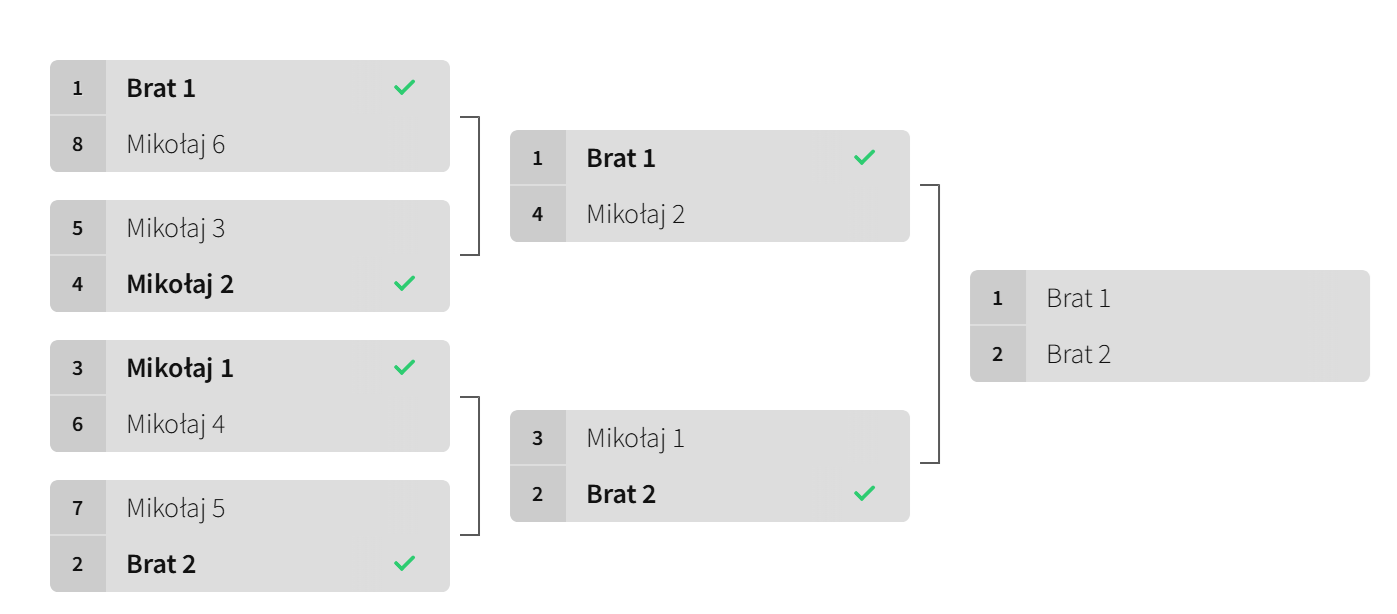
\includegraphics[width=0.7\textwidth]{tasks/12_01.png}

Jest $2^i=4$ miejsc, które prowadzą do pojedynku 3, które wcześniej nie walczą z bratem 1.

Jest $2^n-1=2^3-1=7$ możliwych miejsc dla brata 2 (wszystkie poza miejscem brata 1).

Dodatkowo, aby bracia spotkali się w 3. pojedynku, obaj muszą wygrać swoje wcześniejsze pojedynki (po 2 zwycięstwa każdy), 
co zdarza się z prawdopodobieństwem $\left(\frac12\right)^2 \cdot \left(\frac12\right)^2$.

Stąd w tym przypadku: 
\[P(A_2) = \frac{2^i}{2^n-1} \cdot \left(\frac{1}{2}\right)^i \cdot \left(\frac{1}{2}\right)^i = \frac{4}{7} \cdot \frac{1}{4} \cdot \frac{1}{4} = \frac{1}{28}\]

Ostatecznie zdarzenie $A$, że bracia spotkają się w turnieju, to
\[
A = \bigcup_{i = 0}^{n-1} A_i,
\]
więc
\[
P(A) = \sum_{i = 0}^{n-1} P(A_i) 
= \frac{1}{2^n-1} \sum_{i=0}^{n-1} 2^{-i} 
= \frac{2(1-2^{-n})}{2^n-1} 
= \boxed{2^{1-n}}.
\]

\subsection*{Odpowiedź}
\[
\boxed{2^{1-n}}
\]